\documentclass[titlepage]{article}
\usepackage[pdftex]{graphicx}

% Title
\title{Lab 5: Magnetic Field}
\author{Yacin Nadji}
\date{\today}

\begin{document}
\maketitle

\section{Statement of Objective}\label{sec:obj}
The objective of this lab was to experiment with the effects of magnetic fields, and help to understand the concept of magnetic fields. We specifically dealt with the relationship between magnetic fields and electric currents. We also studied the relationship between the charge, and mass of an electron.

\section{Theory}\label{sec:theory}
Magnetic fields are known to be generated by current loops. You can determine the magnitude of this field using this equation:
\begin{equation}\label{eqn1}
	B(z) = \frac{\mu_0 IR^2 N}{2(R^2 + z^2)^{3/2}}
\end{equation}
When you plot $B$ versus $\frac{1}{(R^2 + z^2)^{3/2}}$ using equation (\ref{eqn1}), the slope is $m = \frac{\mu_0 IR^2 N}{2}$. If you align two identical current loops, you can create a stronger uniform magnetic field. This is essentially what a Helmholtz coil is, and it's magnitude is represented by the following equation:
\begin{equation}\label{eqn2}
	B = \frac{8}{5\sqrt{5}} \frac{\mu_0 IN}{R}
\end{equation}
When $B$ and $I$ are plotted against each other, a slope of $m = \frac{8}{5\sqrt{5}} \frac{\mu_0 N}{R}$ is found. The magnetic force on a wire of length $l$ is described by the following equation:
\begin{equation}\label{eqn3}
	F = I l \times B
\end{equation}

\section{Equipment List}\label{sec:equipment_list}
\begin{itemize}
\item[*] Hall Effect Probe
\item[*] DC Power Source
\item[*] Ammeter
\item[*] Helmholtz Coil
\item[*] Balance
\item[*] Prefab Current Loops
\end{itemize}

\section{Procedure}\label{sec:procedure}
\subsection{Part A: The Hall Effect Probe}\label{sub:part_a_the_hall_effect_probe-proc}
The Hall Effect probe is calibrated by using a permanent magnet of known induction of $750$ Gauss.

\subsection{Part B: Magnetic Field Strength of a Current Loop}\label{sub:part_b_magnetic_field_strength_of_a_current_loop-proc}
A coil of wire is connected to a DC power source to generate current, and thus, a magnetic field. The DC power source generates a current of $1 A$ in the coil. The magnetic field was then measured using a Hall Effect probe. The number of turns in the coil and the radius of the coil were recorded. The magnitude of the magnetic field was recorded multiple times at various distances along the plane of the coil.

\subsection{Part C: Magnetic Field at the Center of a Helmholtz Coil}\label{sub:part_c_magnetic_field_at_the_center_of_a_helmholtz_coil-proc}
Part C is similar to Part B (\S \ref{sub:part_b_magnetic_field_strength_of_a_current_loop-proc}) except it is done with a Helmholtz coil and the current is altered, rather than the position. The radius of the coil, the number of turns, and the magnitude of the magnetic field were all recorded. The Hall Effect probe was placed in the center of the coil.

\subsection{Part D-1: Current Balance - Magnetic Force with Varying Current}\label{sub:part_d_1_current_balance_magnetic_force_with_varying_current-proc}
The current loop with the longest 3­4 section was selected and its length recorded. The loop was then plugged into the main unit with the 3­4 section passing through the pole region of the magnet assembly.  The mass of the magnet was then recorded with no current flowing through the loop, and then at each $0.5A$ increment up to a $4.0A$ maximum.

\subsection{Part D-2: Current Balance - Magnetic Force with Varying Length}\label{sub:part_d_2_current_balance_magnetic_force_with_varying_length-proc}
The setup in Part D­1 (\S \ref{sub:part_d_1_current_balance_magnetic_force_with_varying_current-proc}) was used with the current set to $3.0A$.  The mass was then recorded and the current reduced to naught.  The current loop was then replaced with another loop with a different 3­4 length.  The current was again set to $3.0A$ and the mass recorded.  This procedure was repeated until all of the available current loops were measured.

\section{Data}\label{sec:data}

\subsection{Part B: Magnetic Field Strength of a Current Loop}\label{sub:part_b_magnetic_field_strength_of_a_current_loop-data}
\begin{center}\label{tbl1}
	\textbf{Coil Data}\\
	\begin{tabular}{cc}
	\hline
	Loops $(N)$ & Radius $(m)$\\
	\hline
	104 & 0.0625\\
	\hline
	\end{tabular}
\end{center}\\
\\
\begin{center}\label{tbl2}
	\textbf{Magnetic Field Measurements}\\
	\begin{tabular}{cc}
	\hline
	$z(m)$ & $B$ Gauss\\
	\hline
	0.025 & 19.30\\
	\hline
	0.040 & 17.25\\
	\hline
	0.053 & 15.10\\
	\hline
	0.065 & 13.60\\
	\hline
	0.073 & 11.90\\
	\hline
	0.087 & 10.50\\
	\hline
	0.126 & 8.40\\
	\hline
	0.139 & 8.00\\
	\hline
	0.153 & 7.70\\
	\hline
	0.165 & 7.50\\
	\hline
	0.185 & 7.30\\
	\hline
	\end{tabular}
\end{center}

\subsection{Part C: Magnetic Field at the Center of a Helmholtz Coil}\label{sub:part_c_magnetic_field_at_the_center_of_a_helmholtz_coil-data}

\begin{center}\label{tbl3}
	\textbf{Coil Data}\\
	\begin{tabular}{cc}
	\hline
	Loops $(N)$ & Radius $(m)$\\
	\hline
	104 & 0.0625\\
	\hline
	\end{tabular}
\end{center}\\
\\

\begin{center}\label{tbl4}
	\textbf{Magnetic Field Measurements}\\
	\begin{tabular}{cc}
	\hline
	Current $(A)$ & B (Gauss)\\
	\hline
	0.0 & 7.70\\
	\hline
	0.1 & 9.0\\
	\hline
	0.2 & 10.40\\
	\hline
	0.3 & 12.00\\
	\hline
	0.4 & 13.30\\
	\hline
	0.5 & 14.80\\
	\hline
	0.6 & 16.30\\
	\hline
	0.7 & 17.80\\
	\hline
	0.8 & 19.20\\
	\hline
	0.9 & 20.60\\
	\hline
	1.0 & 22.10\\
	\hline
	\end{tabular}
\end{center}

\subsection{Part D-1: Current Balance - Magnetic Foce with Varying Current}\label{sub:part_d_1_current_balance_magnetic_foce_with_varying_current-data}

\begin{center}\label{tbl5}
	\textbf{Current Loop}\\
	\begin{tabular}{cc}
	\hline
	$l$ & 0.084 m\\
	\hline
	\end{tabular}
\end{center}\\
\\

\begin{center}\label{tbl6}
	\begin{tabular}{cc}
	\hline
	Current $(A)$ & Mass $(kg)$\\
	\hline
	0.0 & 0.1608\\
	\hline
	0.5 & 0.1612\\
	\hline
	1.0 & 0.1615\\
	\hline
	1.5 & 0.1619\\
	\hline
	2.0 & 0.1622\\
	\hline
	2.5 & 0.1626\\
	\hline
	3.0 & 0.1629\\
	\hline
	3.5 & 0.1632\\
	\hline
	4.0 & 0.1636\\
	\hline
	\end{tabular}
\end{center}\\
\\

\subsection{Part D-2: Current Balance - Magnetic Force with Varying Length}\label{sub:part_d_2_current_balance_magnetic_force_with_varying_length-data}

\begin{center}\label{tbl7}
	\textbf{Current Loop}\\
	\begin{tabular}{cc}
	\hline
	Current & 3.0A\\
	\hline
	\end{tabular}
\end{center}\\
\\
\begin{center}\label{tbl8}
	\begin{tabular}{cc}
	\hline
	Length $(m)$ & Mass $(kg)$\\
	\hline
	0.012 & 0.1611\\
	\hline
	0.022 & 0.1614\\
	\hline
	0.032 & 0.1616\\
	\hline
	0.042 & 0.1619\\
	\hline
	0.064 & 0.1623\\
	\hline
	0.084 & 0.1629\\
	\hline
	\end{tabular}
\end{center}

\section{Analysis of Data}\label{sec:analysis_of_data}

\subsection{Part B: Magnetic Field Strench of a Current Loop}\label{sub:part_b_magnetic_field_strench_of_a_current_loop-anl}
Using equation (\ref{eqn1}), we can determine our experimental value of B by making a graph of B vs. $\frac{1}{(R^2 + z^2)^{3/2}}$ as shown in Table \ref{tbl9} and Graph \ref{g1}.

\begin{center}\label{tbl9}
	\textbf{Magnetic Field Measurements}\\
	\begin{tabular}{cccc}
	\hline
	z $(m)$ & B (Gauss) & $B(T)$ & $\frac{1}{(R^2 + z^2)^{3/2}}$\\
	\hline
	0.025 & 19.30 & 0.001930 & 3278.48\\
	\hline
	0.040 & 17.25 & 0.001725 & 2447.46\\
	\hline
	0.053 & 15.10 & 0.001510 & 1817.22\\
	\hline
	0.065 & 13.60 & 0.001360 & 1363.84\\
	\hline
	0.073 & 11.90 & 0.001190 & 1126.75\\
	\hline
	0.087 & 10.50 & 0.001050 & 813.499\\
	\hline
	0.126 & 8.40 & 0.000840 & 359.407\\
	\hline
	0.139 & 8.00 & 0.000800 & 282.490\\
	\hline
	0.153 & 7.70 & 0.000770 & 221.509\\
	\hline
	0.165 & 7.50 & 0.000750 & 182.056\\
	\hline
	0.185 & 7.30 & 0.000730 & 134.301\\
	\hline
	\end{tabular}
\end{center}\\
\\
\begin{center}\label{g1}
	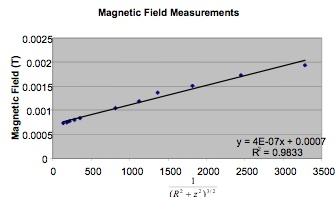
\includegraphics{1.jpg}
\end{center}\\
\\
The slope of the best fit line, as mentioned earlier, is $m = \frac{\mu_0 IR^2 N}{2}$. The theoretical value is $2.55 \times 10^{-7}$ and the experimental value is $4.0 \times 10^{-7}$.

\subsection{Part C: Magnetic Field at the Center of a Helmholtz Coil}\label{sub:part_c_magnetic_field_at_the_center_of_a_helmholtz_coil-anl}
If we use equation (\ref{eqn2}), and the magnetic field measured, we can plot the magnetic field vs. the current.

\begin{center}\label{tbl10}
	\textbf{Magnetic Field Measurements}\\
	\begin{tabular}{ccc}
	\hline
	Current $(A)$ & B (Gauss) & $B(T)$\\
	\hline
	0.0 & 7.70 & 0.000770\\
	\hline
	0.1 & 9.0 & 0.000900\\
	\hline
	0.2 & 10.40 & 0.001040\\
	\hline
	0.3 & 12.00 & 0.001200\\
	\hline
	0.4 & 13.30 & 0.001330\\
	\hline
	0.5 & 14.80 & 0.001480\\
	\hline
	0.6 & 16.30 & 0.001630\\
	\hline
	0.7 & 17.80 & 0.001780\\
	\hline
	0.8 & 19.20 & 0.001920\\
	\hline
	0.9 & 20.60 & 0.002060\\
	\hline
	1.0 & 22.10 & 0.002210\\
	\hline
	\end{tabular}
\end{center}\\
\\
\begin{center}\label{g2}
	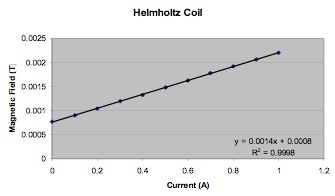
\includegraphics{2.jpg}
\end{center}\\
\\The slope, $m = \frac{8}{5\sqrt{5}} \frac{\mu_0 N}{R}$, has a theoretical value of $0.0015 \frac{T}{A}$ and an experimental value of $0.0014 \frac{T}{A}$.

\subsection{Part D-1: Current Balance - Magnetic Force with Varying Current}\label{sub:part_d_1_current_balance_magnetic_force_with_varying_current-anl}
The change in mass is calculated by subtracting the recorded value for mass from initial value for the mass $(0.1608 kg)$. We then multiply this value by $g$ to get the Force $(N)$.

\begin{center}\label{tbl11}
	\textbf{Current Balance}
	\begin{tabular}{ccc}
	\hline
	Current $(A)$ & Mass $(kg)$ & Force $(N)$\\
	\hline
	0.5 & 0.0004 & 0.0039\\
	\hline
	1.0 & 0.0007 & 0.0069\\
	\hline
	1.5 & 0.0011 & 0.0108\\
	\hline
	2.0 & 0.0014 & 0.0137\\
	\hline
	2.5 & 0.0018 & 0.0177\\
	\hline
	3.0 & 0.0021 & 0.0206\\
	\hline
	3.5 & 0.0024 & 0.0235\\
	\hline
	4.0 & 0.0028 & 0.0275\\
	\hline
	\end{tabular}
\end{center}\\
\\
\begin{center}\label{g3}
	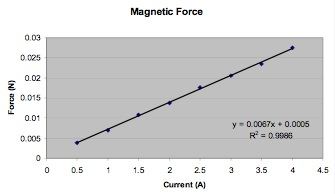
\includegraphics{3.jpg}
\end{center}\\
\\
Graph \ref{g3} has a slope of $m = 0.0067$, being our experimental value, and the theoretical value is $0.0063$. This yields a magnetic field of $0.0798$ teslas.

\subsection{Part D-2: Current Balance - Magnetic Force with Varying Length}\label{sub:part_d_2_current_balance_magnetic_force_with_varying_length-anl}
The process for Section \ref{sub:part_d_2_current_balance_magnetic_force_with_varying_length-anl} is the same as for Section \ref{sub:part_d_1_current_balance_magnetic_force_with_varying_current-anl} but instead of varying the current, we varied the length.

\begin{center}\label{tbl12}
	\begin{tabular}{ccc}
	\hline
	Length $(m)$ & Mass $(kg)$ & Force $(N)$\\
	\hline
	0.012 & 0.0003 & 0.0029\\
	\hline
	0.022 & 0.0006 & 0.0059\\
	\hline
	0.032 & 0.0008 & 0.0078\\
	\hline
	0.042 & 0.0011 & 0.0108\\
	\hline
	0.064 & 0.0015 & 0.0147\\
	\hline
	0.084 & 0.0021 & 0.0206\\
	\hline
	\end{tabular}
\end{center}\\
\\
\begin{center}\label{g4}
	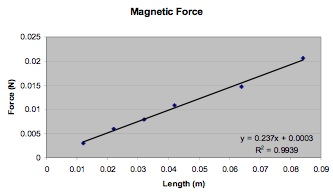
\includegraphics{4.jpg}
\end{center}
The experimental value of the magnetic field is $\frac{m}{I} = \frac{0.237}{3} = 0.079$ teslas.

\section{Question}\label{sec:question}
Parts of segment 2-3 and 4-5 of the current loop are also within the magnetic field of the assembly. Why are we justified in ignoring the force acting on these segments?\\
\\
The forces will cancel themselves out, and they don't act downwards, meaning they do not affect the mass.

\section{Discussion of Results}\label{sec:discussion_of_results}

\subsection{Part B: Magnetic Field Strength of a Current Loop}\label{sub:part_b_magnetic_field_strength_of_a_current_loop-dor}
Our \% error is calculated to be:
\[
	\frac{|4.0 \times 10^{-7}| - |2.55 \times 10^{-7}|}{|2.55 \times 10^{-7}|} * 100 = 36.25\%
\]
which is quite high. The only way this could be achieved is if we calibrated our probe incorrectly.

\subsection{Part C: Magnetic Field at the Center of a Helmholtz Coil}\label{sub:part_c_magnetic_field_at_the_center_of_a_helmholtz_coil-dor}
Our \% error is calculated to be:
\[
	\frac{|0.0014| - |0.0015|}{|0.0015|} * 100 = 7.14\%
\]

\subsection{Part D-1: Current Balance - Magnetic Force with Varying Current}\label{sub:part_d_1_current_balance_magnetic_force_with_varying_current-dor}
Our \% error is calculated to be:
\[
	\frac{|0.0798| - |0.075|}{|0.075|} * 100 = 6.02\%
\]

\subsection{Part D-2: Current Balance - Magnetic Force with Varying Length}\label{sub:part_d_2_current_balance_magnetic_force_with_varying_length-dor}
Our \% error is calculated to be:
\[
	\frac{|0.079| - |0.075|}{|0.075|} * 100 = 5.06\%
\]

\section{Conclusions}\label{sec:conclusions}
All our results turned out very close to what we were looking for, save for Part B. The magnetic field decreases as the distance from the center of the coil increases, going alongside Equation (\ref{eqn1}). Part C showed the relationship between the current and the magnetic field generated. Part D shows the force generated by a magnetic field.

\end{document}